\documentclass{article}

\usepackage{amsmath}
\usepackage{graphicx}
\usepackage{subcaption}
\usepackage{bigfoot}
\usepackage{hyperref}

\title{Project Overview}
\date{5 October 2018}
\author{
	ECE 388
	\\
	\\
	Team 4:
	\\
	Jacob Aubertine
	\\
	Mathieu Bolduc-Clayton
	\\
	Sal Fernandes
}

\begin{document}
	\pagenumbering{gobble}
	\maketitle
	\newpage
	\tableofcontents
	\newpage
	\pagenumbering{arabic}

    \section{Team member contributions}
	    \subsection{Preface}
	    This report may be shorter or less thorough than expected. This is because, as a group, we had agreed to work on different sections in order to even the workload. That did not happen. Instead, this report was almost entirely written by Jacob. Sal  made some edits after the report had been written. Mathieu created the block diagrams in Microsoft Visio. If this had been known to me, or if the other members had contributed equally, this report would likely have been of higher quality.
	    
	    \subsection{Table of contributions}
	    The individual contributions of team members were not measured by time. Instead, a general outline of what each member has done is provided in Table \ref{tab:table1}. The project so far has mostly been broadly designing subsystems, making decisions on how to implement the subsystems, and testing individual components, which all group members have contributed to.
	    \begin{table}[h!]
  	    \begin{center}
            \caption{Team member contributions}
    		\label{tab:table1}
    		\begin{tabular}{r|l}
      			\textbf{Member} & \textbf{Contributions} \\
			    \hline
      			Jacob Aubertine & Wrote entirety of servo motor report and this\\
      			 & report. Will focus on both hardware and software. \\
      			Mathieu Bolduc-Clayton & Created hardware and software block diagrams.\\
      			 & Will focus on hardware.\\
      			Sal Fernandes & Created concept block diagram. Will focus on software.\\
   			\end{tabular}
  	    \end{center}
	\end{table}

	\section{Problem statement}
	The goal of this project is to design and construct a secure private elevator control system. All aspects are to be designed to integrate together as an embedded system. 
	
	The concept block diagram (Figure \ref{fig:concept_block_diagram}, which encompasses both hardware and software, provides a general overview of the elevator's systems. The hardware block diagram (Figure \ref{fig:hardware_block_diagram} provides an overview of just the hardware aspects of the project and they interact with each other. The software block diagram (Figure \ref{fig:software_block_diagram} shows a flowchart of the elevator operations, providing the logic for the system.
	
		% figure
	\begin{figure}[h!]
	    \begin{center}
		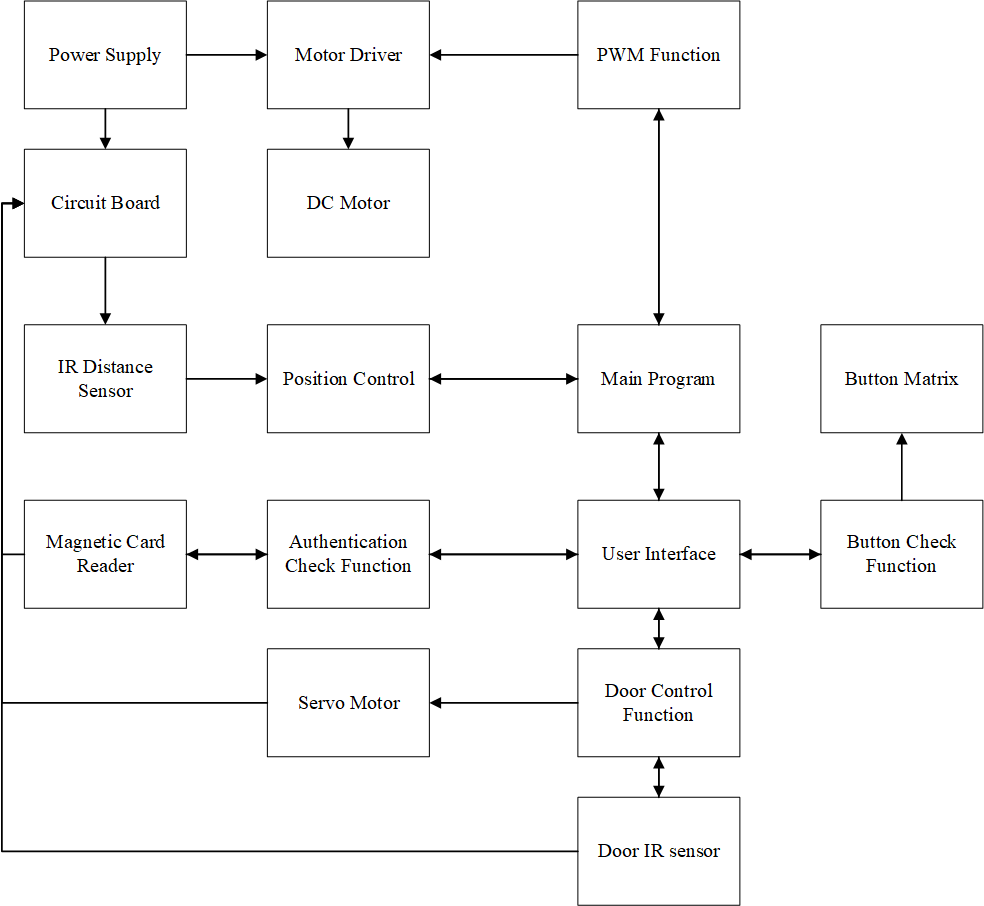
\includegraphics[width=230pt]{cbd.png}
		\caption{Concept block diagram}
		\label{fig:concept_block_diagram}
		\end{center}
	\end{figure}
	
	% figure
	\begin{figure}[h!]
	    \begin{center}
		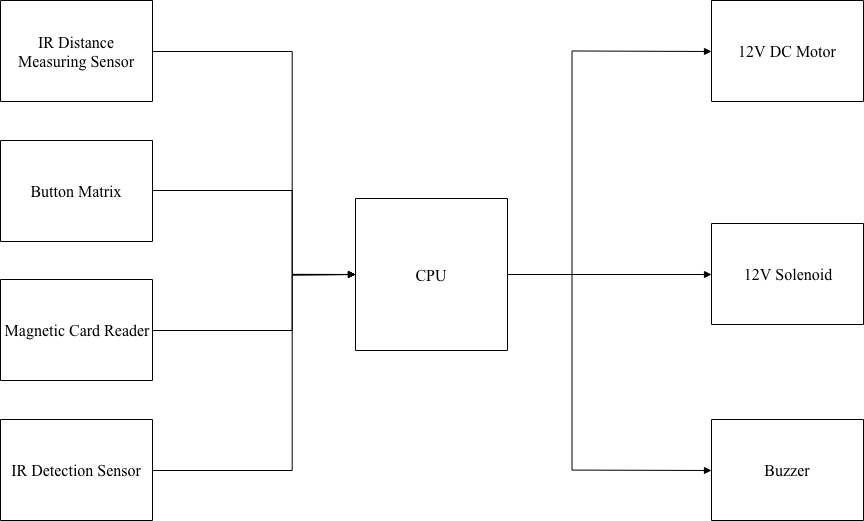
\includegraphics[width=230pt]{hwbd.png}
		\caption{Hardware block diagram}
		\label{fig:hardware_block_diagram}
		\end{center}
	\end{figure}
	
	% figure
	\begin{figure}[h!]
	    \begin{center}
		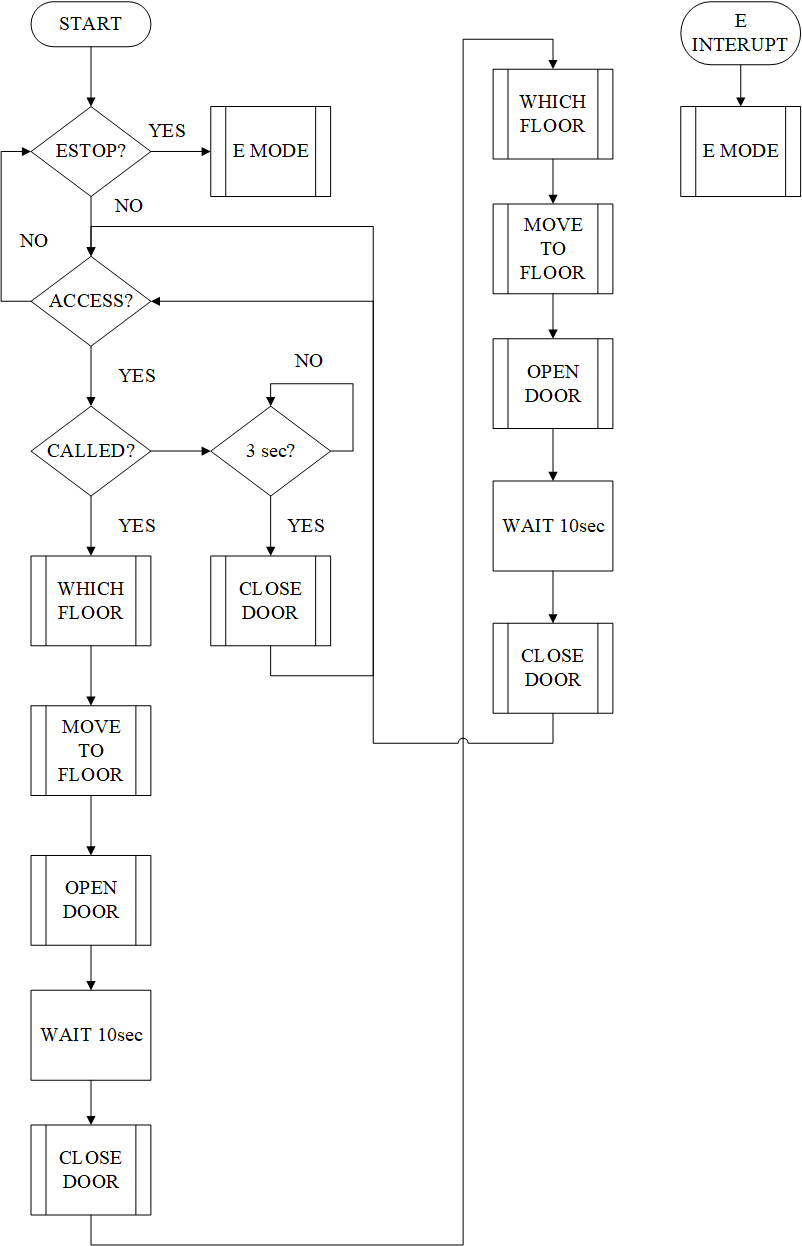
\includegraphics[width=230pt]{swbd.png}
		\caption{Software block diagram}
		\label{fig:software_block_diagram}
		\end{center}
	\end{figure}

	\section{Description of subsystems}
	    \subsection{Height/position}
	    The elevator will be moved by a DC motor connected to a cable that winds and unwinds around a pulley above the shaft in order to bring the elevator up and down. The IR distance sensor measures the distance (using a range of voltages to specify the distance the object is) between the top of the shaft (near the pulley) and the elevator. This allows for knowledge of the elevators position at all times, ensuring it reaches the proper floor. Some sort of track would be ideal to allow the elevator to move smoothly without any unwanted rotation. Unwanted movement would likely disturb the IR sensor's measurements. A buzzer will be used to signify that a floor is reached and the doors are opening.
	    
	    \subsection{Security}
	    A magnetic stripe card reader will be used as the main form of security. It can allow access to individuals if they swipe a valid card. Once a valid card is swiped, they can call the elevator. The elevators doors should stay closed when not in use, so a swipe is required to call the elevator and have its doors open. LED indicators exist on the card reader itself which provide feedback to the user if the swiped card is valid or invalid. The current plan is to use UMass Dartmouth IDs, with a certain number specified as valid.
	    
	    \subsection{Safety}
	    An emergency stop button will exist that halts all function and stops the elevator sounding the buzzer until the button is pressed again. There will be a sensor (assumed to be IR at this point) to detect if there is anything in the way of the open door. If there is something blocking the way, the door is to remain open until the obstruction is no longer there.
	    
	    \subsection{User Interface}
	    Many buttons will be needed for this elevator system. Currently the elevator has four floors. There will need to be a call button on each of these floors (4 total), a button inside the elevator for each floor (4 total), plus an emergency stop button. Altogether, nine buttons are specified. A 4x4 button matrix would give more than enough buttons. If more than the nine are needed, it will be very easy to use the remaining buttons on the matrix. These buttons will be mounted outside of the elevator for testing and easy access.
	    
	    \subsection{Power}
	    Originally, the power was estimated for the solenoid and the stepper motor being using. The DC motor was received very recently and has not been tested, so the power requirements are currently unknown. The stepper and solenoid both ran at 12 V, with the stepper drawing up to 350 mA and the solenoid drawing up to 1 A. Besides the two motors, everything else should be using digital logic. Of these parts, all have run at 5 V.

	\section{Work done so far}
	Thus far, a most of the time spent on this project has been on design and overview. Some components have been tested. The IR distance sensor output a voltage that varies based on how far the infrared beam sensed it traveled. A test was conducted with the sensor supplied 5 V, and the output voltage being measured on the digital multimeter. A meter stick was used to measure the distance, and it was laid flat on the table with the sensor at the 0 cm mark. The datasheet\cite{project_overview:IR_datasheet} stated that a white surface provided the most accurate readings because it was more reflective than darker shades. A notebook was moved at set intervals from the sensor and the voltages were recorded. The results of the test are shown in Table \ref{tab:table2}.
	
    A stepper motor was initially considered for controlling the elevator's height, but since it might not produce smooth movement a DC motor was chosen instead. This has not been tested yet, but it will be once a motor controller is received.
    
    A solenoid motor\cite{project_overview:solenoid_datasheet} was chosen to control the door. Depending on the voltage it can be in one of two linear positions. This provides the two states for the door: open and closed. The motor draws a large amount of current, up to 1 A according to the data-sheet. Transistors are needed to control it, and the transistor used initially was not rated for a high enough current. The TA recommended a transistor array, which allowed multiple transistors to be used (along with ballast resistors) to split up the current traveling through each. The transistor array was a ULN2003\cite{project_overview:uln2003_datasheet}. The circuit diagram showing the solenoid and transistors is in Figure \ref{fig:solenoid}.
    
	% figure
	\begin{figure}[h!]
	    \begin{center}

		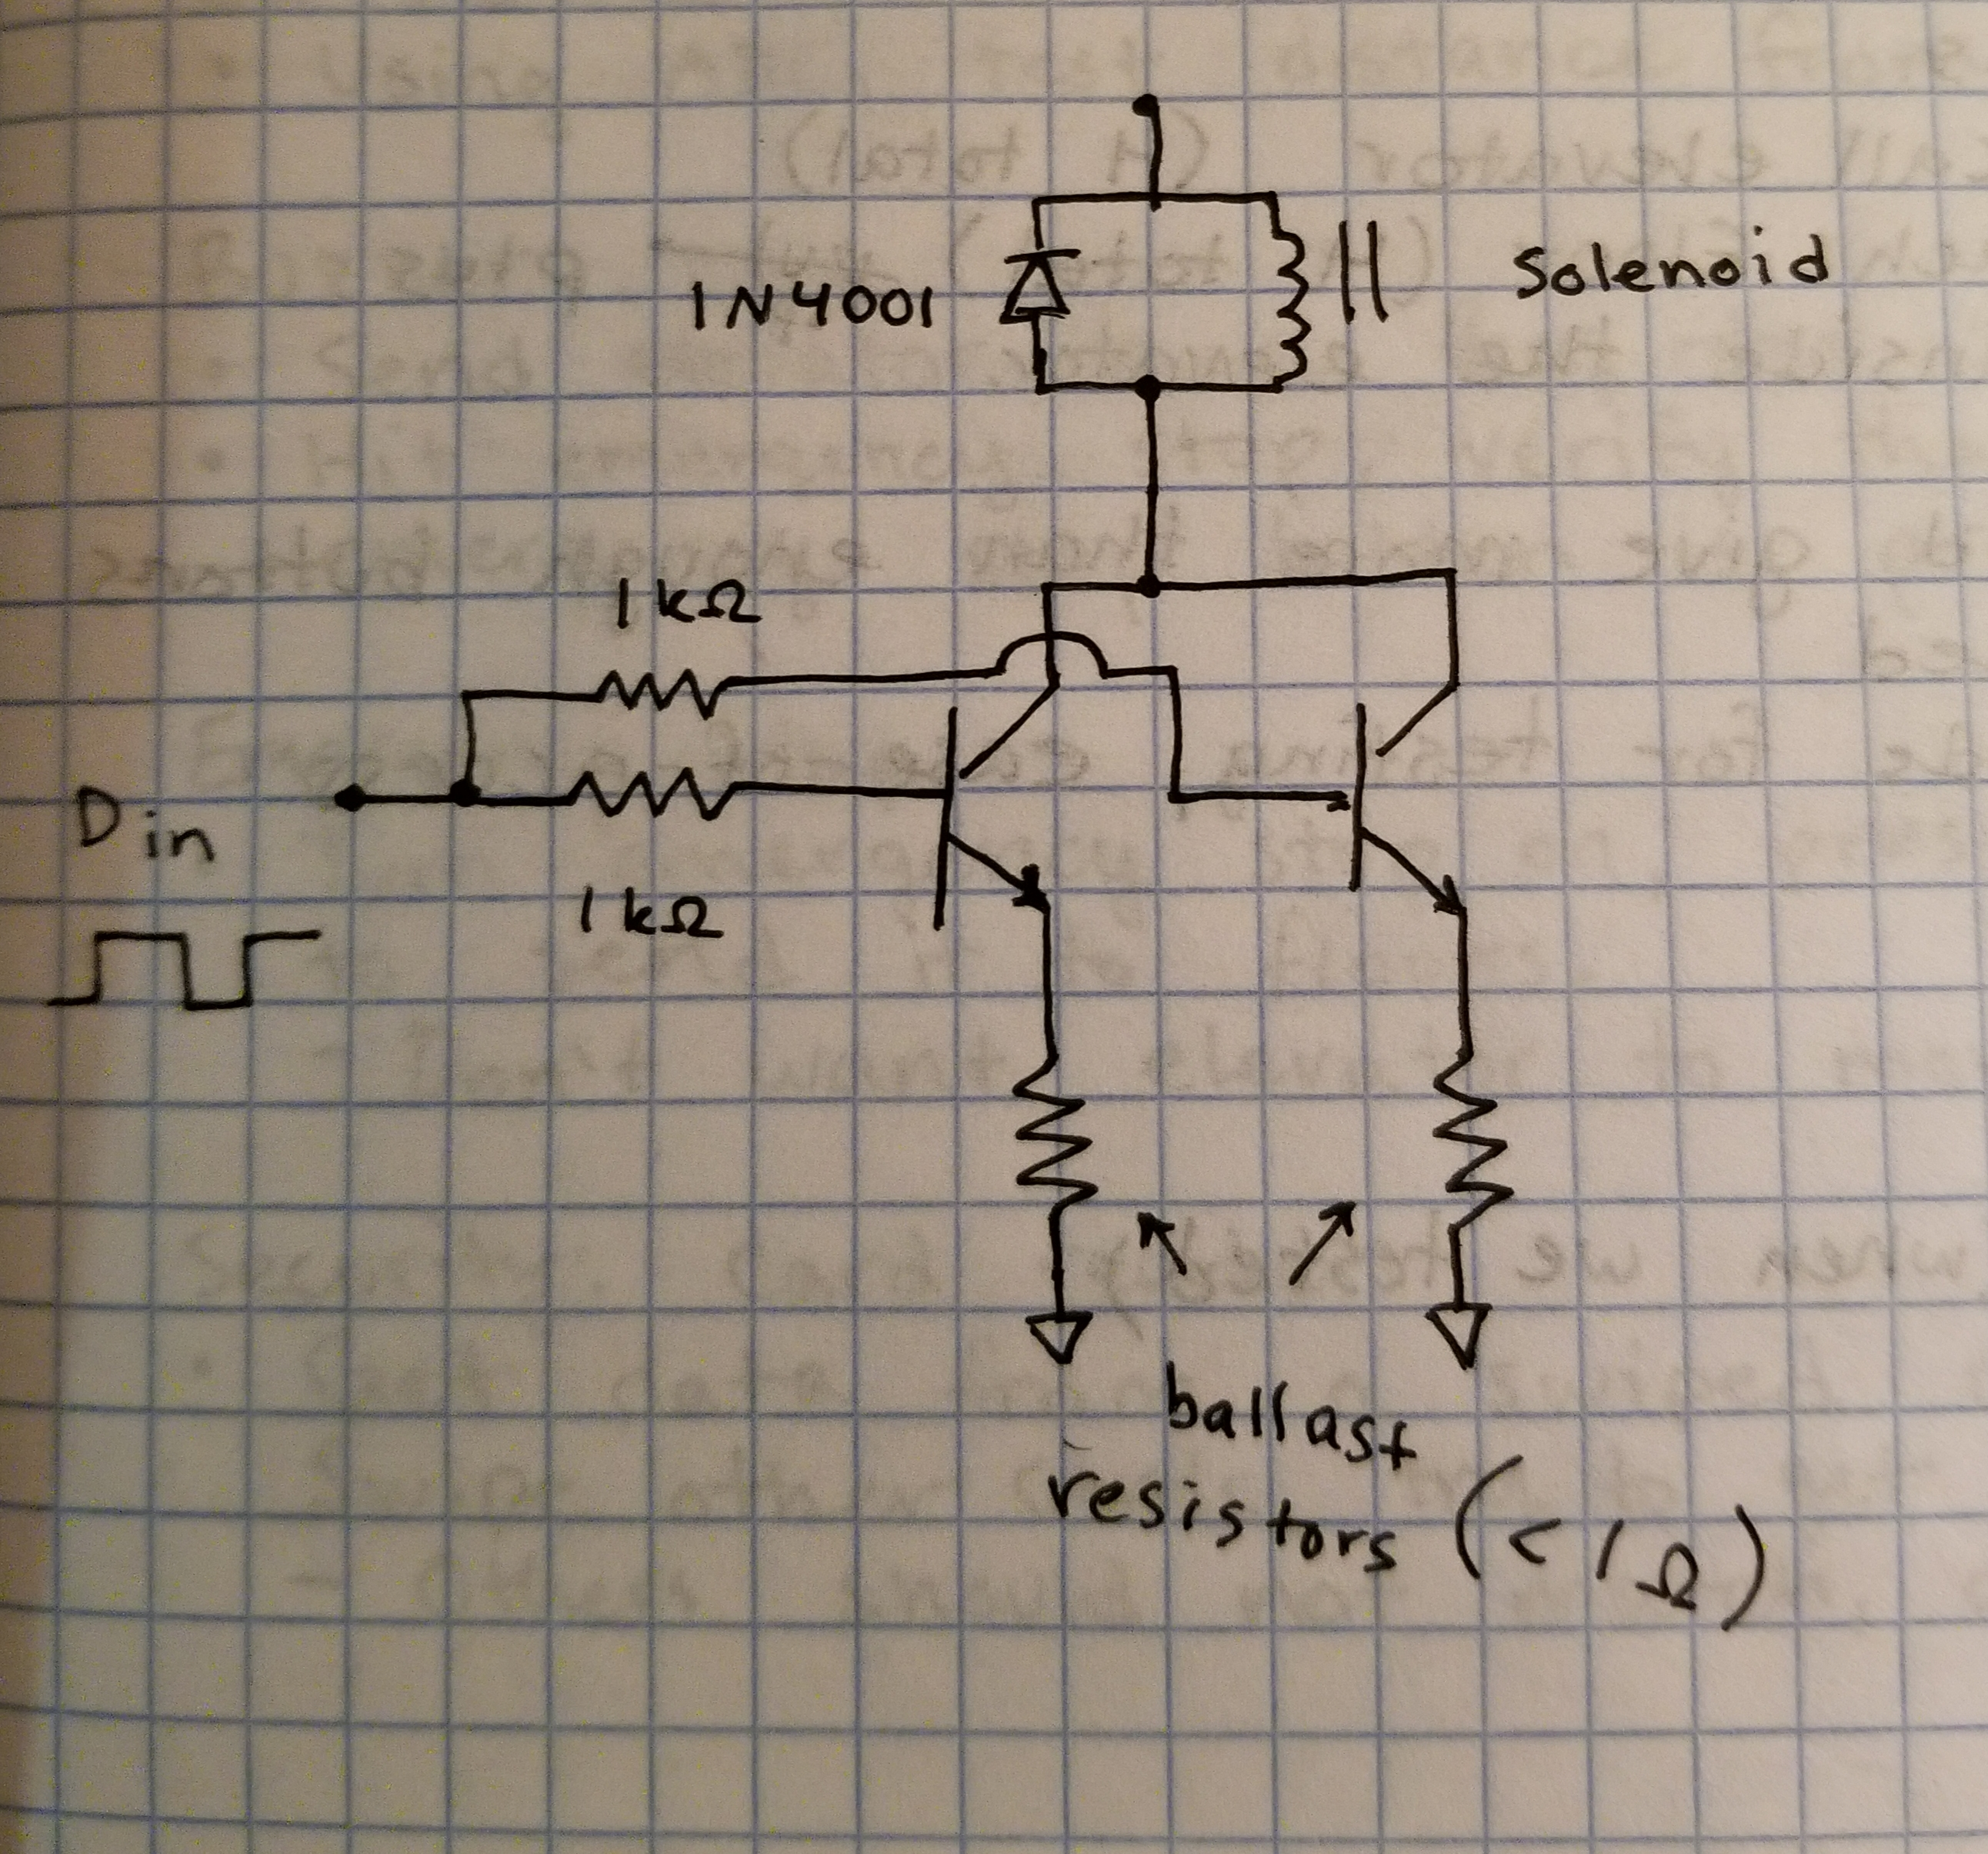
\includegraphics[width=250pt]{solenoid.jpg}
		\caption{Solenoid motor circuit}
		\label{fig:solenoid}
	    \end{center}
	\end{figure}
	
	% table
    \begin{table}[h!]
  	    \begin{center}
            \caption{IR Distance Sensor Voltages}
    		\label{tab:table2}
    		\begin{tabular}{r|r}
      			\textbf{Distance (cm)} & \textbf{Voltage (V)} \\
			    \hline
      			5 & 3.11\\
      			10 & 2.2\\
      			15 & 1.6\\
      			20 & 1.2\\
				25 & 1.0\\
				30 & 0.890 \\
				35 & 0.780 \\
				40 & 0.680 \\
				45 & 0.620 \\
				50 & 0.530 \\
				55 & 0.480 \\
				60 & 0.440 \\
				65 & 0.400 \\
				70 & 0.320 \\
				75 & 0.050 \\
				80 & 0.030 \\
   			\end{tabular}
  	    \end{center}
	\end{table}
	
	
	\section{Future test plans}
	Most of the tests specified involve hardware and software working together. Very few tests, at this point, involve just hardware or just software. The subsections are divided roughly by subsystem or component. Since tests often involve multiple subsystems, they are grouped with what was considered most relevant.
	    \subsection{DC motor}
	    \begin{itemize}
            \item When connected to the motor controller, try making the motor rotate in both directions and verify that it does so.
            \item Measure the time it takes for the elevator to travel from the bottom floor to the top, and top floor to the bottom. These times should be the same. Repeat the measurements with different levels of PWM to determine which speed looks most reasonable.
            \item Using PWN to slow down the speed of the elevator as it approaches the desired floor as to not stop abruptly.  
        \end{itemize}
        
	    \subsection{IR distance sensor}
	    \begin{itemize}
	        \item The sensor by itself had been tested by using a voltmeter to measure its voltage at specific distances.
	        \item After connecting the sensor to the micro controller ADC, test the readings at different distances.
	        \item Record the readings again, this time with the sensor at the top of the elevator shaft. Get positions for each floor based on the distance from the sensor.
	        \item Once the positions are known, have the elevator travel to each floor from above and below (if possible) to measure how far the elevator is physically from the desired position. The elevator should line up from both directions.
	        \item Set a distance for the motor to stop at, and see how long it takes for it to stop, and record how far it stopped from the desired location.
	    \end{itemize}
	    
	    \subsection{Buzzer}
	    \begin{itemize}
	        \item Observe the timer output from the micro-controller and verify that the frequency of the waveform matches what was specified.
	        \item Send the elevator to a floor and verify that the buzzer buzzes when it reaches the floor.
	        \item Press the emergency stop button, verify that the buzzer buzzes until the button is pressed again.
	    \end{itemize}
	    
	    \subsection{Emergency stop}
	    \begin{itemize}
	        \item Press emergency stop to stop elevator. Try to press buttons to call elevator and send it to another floor. The elevator should not move until the emergency stop is disengaged.
	    \end{itemize}
	    
	    \subsection{Security: magnetic stripe reader}
	    \begin{itemize}
	        \item With the reader connected to the micro-controller, record the data received from swiping a card. This card and its data will be considered valid. Try to get a match by swiping other cards. Ideally they should not match and should be rejected.
	        \item The elevator should not be called until a valid card is swiped. Try different input combinations to move elevator or open a door before a valid card is swiped. Also try this when an invalid card is swiped. Repeat the same tests by swiping a valid card and ensure that the doors open and the elevator does move (if not on the floor).
	    \end{itemize}
	    
	    \subsection{Door}
	    \begin{itemize}
	        \item The door should open shortly after a floor is reached. This time will be measured and adjusted as necessary, and must be after the elevator stops moving.
	        \item The door should then close some time after a floor is reached and remained closed until a valid card is swiped. This time will also be measured and adjusted to ensure passengers have enough time to safely exit the elevator.
	        \item The door should remain closed while moving, and the elevator should continue to its destination before moving to another floor. The call buttons should be pressed for different floors while the elevator is moving to make sure it continues and the doors remain closed until stopped.
	        \item If at a floor with the door open and something is detecting in the path of the door, the door should remain open and the elevator should not move until the path is clear for a time. The call buttons should be pressed while the path is blocked to test if the elevator does actually move. The time it takes the door to close after the path has been cleared will be measured to ensure it can safely be cleared and remain clear.
	    \end{itemize}
	    
	    \subsection{Buttons}
	    \begin{itemize}
	        \item The button matrix should be tested independently to ensure every button can be properly detected.
	        \item The emergency stop button should halt all function and continue to until it is pressed again. This should be tested when the elevator is in different positions, such as when it is moving between floors and stopped at a floor.
	    \end{itemize}
	    
	    \newpage
	    \nocite{*}
        \bibliographystyle{IEEEtran}
        \bibliography{project_overview}
\end{document}